% Options for packages loaded elsewhere
\PassOptionsToPackage{unicode}{hyperref}
\PassOptionsToPackage{hyphens}{url}
\PassOptionsToPackage{dvipsnames,svgnames,x11names}{xcolor}
%
\documentclass[
  a4paper,
  DIV=11,
  numbers=noendperiod,
  oneside]{scrreprt}

\usepackage{amsmath,amssymb}
\usepackage{iftex}
\ifPDFTeX
  \usepackage[T1]{fontenc}
  \usepackage[utf8]{inputenc}
  \usepackage{textcomp} % provide euro and other symbols
\else % if luatex or xetex
  \usepackage{unicode-math}
  \defaultfontfeatures{Scale=MatchLowercase}
  \defaultfontfeatures[\rmfamily]{Ligatures=TeX,Scale=1}
\fi
\usepackage{lmodern}
\ifPDFTeX\else  
    % xetex/luatex font selection
\fi
% Use upquote if available, for straight quotes in verbatim environments
\IfFileExists{upquote.sty}{\usepackage{upquote}}{}
\IfFileExists{microtype.sty}{% use microtype if available
  \usepackage[]{microtype}
  \UseMicrotypeSet[protrusion]{basicmath} % disable protrusion for tt fonts
}{}
\makeatletter
\@ifundefined{KOMAClassName}{% if non-KOMA class
  \IfFileExists{parskip.sty}{%
    \usepackage{parskip}
  }{% else
    \setlength{\parindent}{0pt}
    \setlength{\parskip}{6pt plus 2pt minus 1pt}}
}{% if KOMA class
  \KOMAoptions{parskip=half}}
\makeatother
\usepackage{xcolor}
\usepackage[left=1in,marginparwidth=2.0in,textwidth=4.0in,marginparsep=0.3in]{geometry}
\setlength{\emergencystretch}{3em} % prevent overfull lines
\setcounter{secnumdepth}{-\maxdimen} % remove section numbering
% Make \paragraph and \subparagraph free-standing
\ifx\paragraph\undefined\else
  \let\oldparagraph\paragraph
  \renewcommand{\paragraph}[1]{\oldparagraph{#1}\mbox{}}
\fi
\ifx\subparagraph\undefined\else
  \let\oldsubparagraph\subparagraph
  \renewcommand{\subparagraph}[1]{\oldsubparagraph{#1}\mbox{}}
\fi

\usepackage{color}
\usepackage{fancyvrb}
\newcommand{\VerbBar}{|}
\newcommand{\VERB}{\Verb[commandchars=\\\{\}]}
\DefineVerbatimEnvironment{Highlighting}{Verbatim}{commandchars=\\\{\}}
% Add ',fontsize=\small' for more characters per line
\usepackage{framed}
\definecolor{shadecolor}{RGB}{241,243,245}
\newenvironment{Shaded}{\begin{snugshade}}{\end{snugshade}}
\newcommand{\AlertTok}[1]{\textcolor[rgb]{0.68,0.00,0.00}{#1}}
\newcommand{\AnnotationTok}[1]{\textcolor[rgb]{0.37,0.37,0.37}{#1}}
\newcommand{\AttributeTok}[1]{\textcolor[rgb]{0.40,0.45,0.13}{#1}}
\newcommand{\BaseNTok}[1]{\textcolor[rgb]{0.68,0.00,0.00}{#1}}
\newcommand{\BuiltInTok}[1]{\textcolor[rgb]{0.00,0.23,0.31}{#1}}
\newcommand{\CharTok}[1]{\textcolor[rgb]{0.13,0.47,0.30}{#1}}
\newcommand{\CommentTok}[1]{\textcolor[rgb]{0.37,0.37,0.37}{#1}}
\newcommand{\CommentVarTok}[1]{\textcolor[rgb]{0.37,0.37,0.37}{\textit{#1}}}
\newcommand{\ConstantTok}[1]{\textcolor[rgb]{0.56,0.35,0.01}{#1}}
\newcommand{\ControlFlowTok}[1]{\textcolor[rgb]{0.00,0.23,0.31}{#1}}
\newcommand{\DataTypeTok}[1]{\textcolor[rgb]{0.68,0.00,0.00}{#1}}
\newcommand{\DecValTok}[1]{\textcolor[rgb]{0.68,0.00,0.00}{#1}}
\newcommand{\DocumentationTok}[1]{\textcolor[rgb]{0.37,0.37,0.37}{\textit{#1}}}
\newcommand{\ErrorTok}[1]{\textcolor[rgb]{0.68,0.00,0.00}{#1}}
\newcommand{\ExtensionTok}[1]{\textcolor[rgb]{0.00,0.23,0.31}{#1}}
\newcommand{\FloatTok}[1]{\textcolor[rgb]{0.68,0.00,0.00}{#1}}
\newcommand{\FunctionTok}[1]{\textcolor[rgb]{0.28,0.35,0.67}{#1}}
\newcommand{\ImportTok}[1]{\textcolor[rgb]{0.00,0.46,0.62}{#1}}
\newcommand{\InformationTok}[1]{\textcolor[rgb]{0.37,0.37,0.37}{#1}}
\newcommand{\KeywordTok}[1]{\textcolor[rgb]{0.00,0.23,0.31}{#1}}
\newcommand{\NormalTok}[1]{\textcolor[rgb]{0.00,0.23,0.31}{#1}}
\newcommand{\OperatorTok}[1]{\textcolor[rgb]{0.37,0.37,0.37}{#1}}
\newcommand{\OtherTok}[1]{\textcolor[rgb]{0.00,0.23,0.31}{#1}}
\newcommand{\PreprocessorTok}[1]{\textcolor[rgb]{0.68,0.00,0.00}{#1}}
\newcommand{\RegionMarkerTok}[1]{\textcolor[rgb]{0.00,0.23,0.31}{#1}}
\newcommand{\SpecialCharTok}[1]{\textcolor[rgb]{0.37,0.37,0.37}{#1}}
\newcommand{\SpecialStringTok}[1]{\textcolor[rgb]{0.13,0.47,0.30}{#1}}
\newcommand{\StringTok}[1]{\textcolor[rgb]{0.13,0.47,0.30}{#1}}
\newcommand{\VariableTok}[1]{\textcolor[rgb]{0.07,0.07,0.07}{#1}}
\newcommand{\VerbatimStringTok}[1]{\textcolor[rgb]{0.13,0.47,0.30}{#1}}
\newcommand{\WarningTok}[1]{\textcolor[rgb]{0.37,0.37,0.37}{\textit{#1}}}

\providecommand{\tightlist}{%
  \setlength{\itemsep}{0pt}\setlength{\parskip}{0pt}}\usepackage{longtable,booktabs,array}
\usepackage{calc} % for calculating minipage widths
% Correct order of tables after \paragraph or \subparagraph
\usepackage{etoolbox}
\makeatletter
\patchcmd\longtable{\par}{\if@noskipsec\mbox{}\fi\par}{}{}
\makeatother
% Allow footnotes in longtable head/foot
\IfFileExists{footnotehyper.sty}{\usepackage{footnotehyper}}{\usepackage{footnote}}
\makesavenoteenv{longtable}
\usepackage{graphicx}
\makeatletter
\def\maxwidth{\ifdim\Gin@nat@width>\linewidth\linewidth\else\Gin@nat@width\fi}
\def\maxheight{\ifdim\Gin@nat@height>\textheight\textheight\else\Gin@nat@height\fi}
\makeatother
% Scale images if necessary, so that they will not overflow the page
% margins by default, and it is still possible to overwrite the defaults
% using explicit options in \includegraphics[width, height, ...]{}
\setkeys{Gin}{width=\maxwidth,height=\maxheight,keepaspectratio}
% Set default figure placement to htbp
\makeatletter
\def\fps@figure{htbp}
\makeatother
\newlength{\cslhangindent}
\setlength{\cslhangindent}{1.5em}
\newlength{\csllabelwidth}
\setlength{\csllabelwidth}{3em}
\newlength{\cslentryspacingunit} % times entry-spacing
\setlength{\cslentryspacingunit}{\parskip}
\newenvironment{CSLReferences}[2] % #1 hanging-ident, #2 entry spacing
 {% don't indent paragraphs
  \setlength{\parindent}{0pt}
  % turn on hanging indent if param 1 is 1
  \ifodd #1
  \let\oldpar\par
  \def\par{\hangindent=\cslhangindent\oldpar}
  \fi
  % set entry spacing
  \setlength{\parskip}{#2\cslentryspacingunit}
 }%
 {}
\usepackage{calc}
\newcommand{\CSLBlock}[1]{#1\hfill\break}
\newcommand{\CSLLeftMargin}[1]{\parbox[t]{\csllabelwidth}{#1}}
\newcommand{\CSLRightInline}[1]{\parbox[t]{\linewidth - \csllabelwidth}{#1}\break}
\newcommand{\CSLIndent}[1]{\hspace{\cslhangindent}#1}

\usepackage{amsmath, amssymb}
\KOMAoption{captions}{tablesignature}
\makeatletter
\makeatother
\makeatletter
\makeatother
\makeatletter
\@ifpackageloaded{caption}{}{\usepackage{caption}}
\AtBeginDocument{%
\ifdefined\contentsname
  \renewcommand*\contentsname{Table of contents}
\else
  \newcommand\contentsname{Table of contents}
\fi
\ifdefined\listfigurename
  \renewcommand*\listfigurename{List of Figures}
\else
  \newcommand\listfigurename{List of Figures}
\fi
\ifdefined\listtablename
  \renewcommand*\listtablename{List of Tables}
\else
  \newcommand\listtablename{List of Tables}
\fi
\ifdefined\figurename
  \renewcommand*\figurename{Figure}
\else
  \newcommand\figurename{Figure}
\fi
\ifdefined\tablename
  \renewcommand*\tablename{Table}
\else
  \newcommand\tablename{Table}
\fi
}
\@ifpackageloaded{float}{}{\usepackage{float}}
\floatstyle{ruled}
\@ifundefined{c@chapter}{\newfloat{codelisting}{h}{lop}}{\newfloat{codelisting}{h}{lop}[chapter]}
\floatname{codelisting}{Listing}
\newcommand*\listoflistings{\listof{codelisting}{List of Listings}}
\makeatother
\makeatletter
\@ifpackageloaded{caption}{}{\usepackage{caption}}
\@ifpackageloaded{subcaption}{}{\usepackage{subcaption}}
\makeatother
\makeatletter
\@ifpackageloaded{tcolorbox}{}{\usepackage[skins,breakable]{tcolorbox}}
\makeatother
\makeatletter
\@ifundefined{shadecolor}{\definecolor{shadecolor}{rgb}{.97, .97, .97}}
\makeatother
\makeatletter
\makeatother
\makeatletter
\@ifpackageloaded{sidenotes}{}{\usepackage{sidenotes}}
\@ifpackageloaded{marginnote}{}{\usepackage{marginnote}}
\makeatother
\makeatletter
\makeatother
\ifLuaTeX
  \usepackage{selnolig}  % disable illegal ligatures
\fi
\IfFileExists{bookmark.sty}{\usepackage{bookmark}}{\usepackage{hyperref}}
\IfFileExists{xurl.sty}{\usepackage{xurl}}{} % add URL line breaks if available
\urlstyle{same} % disable monospaced font for URLs
\hypersetup{
  pdftitle={Solving ODEs and ODE systems},
  colorlinks=true,
  linkcolor={blue},
  filecolor={Maroon},
  citecolor={Blue},
  urlcolor={Blue},
  pdfcreator={LaTeX via pandoc}}

\title{Solving ODEs and ODE systems}
\author{}
\date{}

\begin{document}
\maketitle
\ifdefined\Shaded\renewenvironment{Shaded}{\begin{tcolorbox}[enhanced, boxrule=0pt, borderline west={3pt}{0pt}{shadecolor}, frame hidden, interior hidden, sharp corners, breakable]}{\end{tcolorbox}}\fi

Solving Ordinary Differential Equations is one of the most common use
cases for scientific computing in engineering applications.

The Julia package
\href{https://docs.sciml.ai/DiffEqDocs/stable/}{DifferentialEquations.jl}
is one of the biggest selling points of the language. It offers an
unparalled range of solvers, all using the same interface\sidenote{\footnotesize So
  changing the solver does not require any changes in the definition of
  the problem, even when moving between ODEs, DAEs and SDAEs.}.

\hypertarget{example-4-element-windkessel-model}{%
\section{Example: 4-Element Windkessel
Model}\label{example-4-element-windkessel-model}}

The windkessel model is a common model for the pressure response of the
vascular system (blood circulation) to a periodic, pulsing flow waveform
(Westerhof et al.
2019)\marginpar{\begin{footnotesize}\leavevmode\vadjust pre{\protect\hypertarget{ref-Westerhof2019}{}}%
Westerhof, Nicolaas, Nikolaos Stergiopulos, Mark I. M. Noble, and Berend
E. Westerhof. 2019. \emph{Snapshots of {Hemodynamics}: {An Aid} for
{Clinical Research} and {Graduate Education}}. {Cham}: {Springer
International Publishing}.
\url{https://doi.org/10.1007/978-3-319-91932-4}.\vspace{2mm}\par\end{footnotesize}}.

Here we are going to work with the 4-Element windkessel model
(Stergiopulos, Westerhof, and Westerhof
1999)\marginpar{\begin{footnotesize}\leavevmode\vadjust pre{\protect\hypertarget{ref-Stergiopulos1999}{}}%
Stergiopulos, Nikos, Berend E. Westerhof, and Nico Westerhof. 1999.
{``Total Arterial Inertance as the Fourth Element of the Windkessel
Model.''} \emph{American Journal of Physiology-Heart and Circulatory
Physiology} 276 (1): H81--88.
\url{https://doi.org/10.1152/ajpheart.1999.276.1.H81}.\vspace{2mm}\par\end{footnotesize}},
comprising a flow source (time dependent flow rate), two resistors for
characteristic Resistance of the near vessel (aorta), \(R_{c}\), and
systemic (peripheral) resistance, \(R_{p}\), a compliance (capacitance)
\(C\), representing the blood storage capacity of the peripheral
vessels, and an inductance \(L_p\), representing the inertia in the
proximal, large vessel, e.g., the aorta.

The pressures in this circuit - \(p_{1}\) before, and \(p_{2}\) after
the proximal L-R element - are described by the system of ODEs:

\begin{equation}\protect\hypertarget{eq-wk4-1}{}{
\frac{d p_{1}}{d t}  =  - \frac{R_{c}}{L_{p}} p_{1} + \left( \frac{R_{c}}{L_{p}} - \frac{1}{R_{p} C} \right) p_{2} 
+ R_{c} \frac{d I(t)}{d t} + \frac{I(t)}{C} 
}\label{eq-wk4-1}\end{equation}

\begin{equation}\protect\hypertarget{eq-wk4-2}{}{
\frac{d p_{2}}{d t}  =  - \frac{1}{R_{p} C} p_{2} + \frac{I(t)}{C} 
}\label{eq-wk4-2}\end{equation}

\begin{figure}

\sidecaption{\label{fig-4wk}4-Element Windkessel Model}

{\centering \includegraphics{ODEsolver_files/mediabag/images/images_for_ODEsolver.qmd/wk4.drawio.pdf}

}

\end{figure}

In order to implement this model, we need to load the required modules.
We use \texttt{DifferentialEquations}, \texttt{Plots}, and
\texttt{ForwardDiff} for the time-derivative
\(\frac{\partial I}{\partial t}\):

\begin{Shaded}
\begin{Highlighting}[]
\ImportTok{using} \BuiltInTok{DifferentialEquations}\NormalTok{, }\BuiltInTok{ForwardDiff}\NormalTok{, }\BuiltInTok{Plots}
\end{Highlighting}
\end{Shaded}

The input waveform is a generic half-period of a sine-wave with a
systolic (ejection) time of \(t_{syst} = 0.4 T\), with
\(T=1\ \mathrm{s}\) period-time (60 beats per minute). The dicrotic
notch is modelled by running the sine into the negative for
\(t_{dicr} = 0.03\ \mathrm{s}\):

\begin{equation}
    I = 
    \begin{cases}
        I_{min} + (I_{max} - I_{min})  \sin \left(\frac{\pi}{t_{syst}} t \right) & \text{if } t < (t_{syst} + t_{dicr})\\
        I_{min} & \text{else} 
    \end{cases}
\end{equation}

In Julia, this function is implemented as\sidenote{\footnotesize Note that we use type
  specifications to define the parameters. Julia does suffer in
  performance, when untyped global variables are used, since these break
  type stability in the multiple dispatch. Making these parameter
  constant fixes their type. We should really be using these parameters
  in the function definition, or use a lambda function. But a lambda
  function is slower than typed variables.}:

\begin{Shaded}
\begin{Highlighting}[]
\CommentTok{\# max and min volume flow in ml/s}
\NormalTok{max\_i}\OperatorTok{::}\DataTypeTok{Float64 }\OperatorTok{=} \FloatTok{425}
\NormalTok{min\_i}\OperatorTok{::}\DataTypeTok{Float64 }\OperatorTok{=} \FloatTok{0.0}

\CommentTok{\# period time}
\NormalTok{T}\OperatorTok{::}\DataTypeTok{Float64 }\OperatorTok{=} \FloatTok{1.0}

\CommentTok{\# Syst. Time in s}
\NormalTok{systTime}\OperatorTok{::}\DataTypeTok{Float64 }\OperatorTok{=} \FloatTok{2} \OperatorTok{/} \FloatTok{5} \OperatorTok{*}\NormalTok{ T}

\CommentTok{\# Dicrotic notch time in s}
\NormalTok{dicrTime}\OperatorTok{::}\DataTypeTok{Float64 }\OperatorTok{=} \FloatTok{0.03}

\KeywordTok{function} \FunctionTok{I}\NormalTok{(t)}
    \CommentTok{\# implicit conditional using boolean multiplicator}
    \CommentTok{\# sine waveform}
\NormalTok{    t }\OperatorTok{=}\NormalTok{ t }\OperatorTok{{-}}\NormalTok{ T }\OperatorTok{*}\NormalTok{ (t }\OperatorTok{÷}\NormalTok{ T)}

    \ControlFlowTok{return}\NormalTok{ ((max\_i }\OperatorTok{{-}}\NormalTok{ min\_i) }\OperatorTok{*} \FunctionTok{sin}\NormalTok{(}\ConstantTok{pi} \OperatorTok{/}\NormalTok{ systTime }\OperatorTok{*}\NormalTok{ (t))}
            \OperatorTok{*}\NormalTok{ (t }\OperatorTok{\textless{}}\NormalTok{ (systTime }\OperatorTok{+}\NormalTok{ dicrTime) )}
            \OperatorTok{+}\NormalTok{ min\_i)}
\KeywordTok{end} 
\end{Highlighting}
\end{Shaded}

We can quickly plot this function in Figure~\ref{fig-igen}.

\begin{Shaded}
\begin{Highlighting}[]
\NormalTok{plotTime }\OperatorTok{=} \FunctionTok{LinRange}\NormalTok{(}\FloatTok{0}\NormalTok{,}\FloatTok{1}\NormalTok{,}\FloatTok{100}\NormalTok{)}

\FunctionTok{plot}\NormalTok{(plotTime, }\FunctionTok{I}\NormalTok{.(plotTime),}
\NormalTok{     xlabel }\OperatorTok{=} \StringTok{"t [s]"}\NormalTok{, ylabel }\OperatorTok{=} \StringTok{"I [ml s\textless{}sup\textgreater{}{-}1\textless{}/sup\textgreater{}]"}\NormalTok{, label }\OperatorTok{=} \StringTok{"Outflow"}\NormalTok{) }
\end{Highlighting}
\end{Shaded}

\begin{figure}[H]

\sidecaption{\label{fig-igen}Generic waveform, representing ejection of
blood from left ventricle in the aorta, including dicrotic notch
(backflow at valve closure).}

{\centering 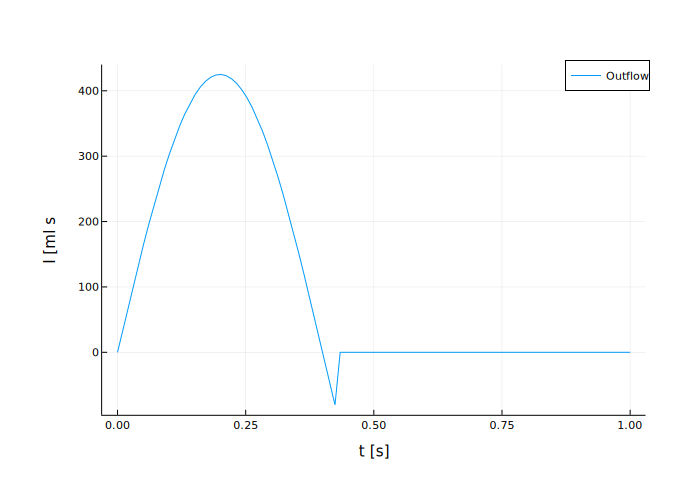
\includegraphics{ODEsolver_files/mediabag/ODEsolver_files/figure-pdf/fig-igen-output-1.pdf}

}

\end{figure}

The definition of the ODEs Equation~\ref{eq-wk4-1} and
Equation~\ref{eq-wk4-2} is done as a function with parameters
\texttt{dP} and \texttt{P}, for \(\frac{d p_{1,2}}{d t}\), and
\(p_{1,2}\), respectively\sidenote{\footnotesize \texttt{P} is a vector of values,
  actually, as is \texttt{dP}.}

\begin{Shaded}
\begin{Highlighting}[]
\KeywordTok{function} \FunctionTok{wk4}\NormalTok{(dP, P, params, t)}

\NormalTok{    Rc, Rp, C, Lp }\OperatorTok{=}\NormalTok{ params}

\NormalTok{    dP[}\FloatTok{1}\NormalTok{] }\OperatorTok{=}\NormalTok{ (}
        \OperatorTok{{-}}\NormalTok{Rc }\OperatorTok{/}\NormalTok{ Lp }\OperatorTok{*}\NormalTok{ P[}\FloatTok{1}\NormalTok{]}
        \OperatorTok{+}\NormalTok{ (Rc }\OperatorTok{/}\NormalTok{ Lp }\OperatorTok{{-}} \FloatTok{1} \OperatorTok{/}\NormalTok{ Rp }\OperatorTok{/}\NormalTok{ C) }\OperatorTok{*}\NormalTok{ P[}\FloatTok{2}\NormalTok{]}
        \OperatorTok{+}\NormalTok{ Rc }\OperatorTok{*}\NormalTok{ ForwardDiff.}\FunctionTok{derivative}\NormalTok{(I, t)}
        \OperatorTok{+} \FunctionTok{I}\NormalTok{(t) }\OperatorTok{/}\NormalTok{ C}
\NormalTok{        )}

\NormalTok{    dP[}\FloatTok{2}\NormalTok{] }\OperatorTok{=} \OperatorTok{{-}}\FloatTok{1} \OperatorTok{/}\NormalTok{ Rp }\OperatorTok{/}\NormalTok{ C }\OperatorTok{*}\NormalTok{ P[}\FloatTok{2}\NormalTok{] }\OperatorTok{+} \FunctionTok{I}\NormalTok{(t) }\OperatorTok{/}\NormalTok{ C}

    \ControlFlowTok{return}\NormalTok{ dP[}\FloatTok{1}\NormalTok{], dP[}\FloatTok{2}\NormalTok{]}

\KeywordTok{end}
\end{Highlighting}
\end{Shaded}

We define the parameters, initial conditions, and time span for the
integration:

\begin{Shaded}
\begin{Highlighting}[]
\NormalTok{Rc }\OperatorTok{=} \FloatTok{0.03}
\NormalTok{Rp }\OperatorTok{=} \FloatTok{1.0}
\NormalTok{C  }\OperatorTok{=} \FloatTok{2.0}
\NormalTok{Lp }\OperatorTok{=} \FloatTok{0.02}

\NormalTok{tspan }\OperatorTok{=}\NormalTok{ (}\FloatTok{0}\NormalTok{, }\FloatTok{10}\NormalTok{)}

\NormalTok{params }\OperatorTok{=}\NormalTok{ [Rc, Rp, C, Lp]}

\NormalTok{P0 }\OperatorTok{=} \FunctionTok{zeros}\NormalTok{(}\FloatTok{2}\NormalTok{)}
\end{Highlighting}
\end{Shaded}

{
\makeatletter
\def\LT@makecaption#1#2#3{%
  \noalign{\smash{\hbox{\kern\textwidth\rlap{\kern\marginparsep
  \parbox[t]{\marginparwidth}{%
    \footnotesize{%
      \vspace{(1.1\baselineskip)}
    #1{#2: }\ignorespaces #3}}}}}}%
    }
\makeatother

\begin{verbatim}
2-element Vector{Float64}:
 0.0
 0.0
\end{verbatim}

}

And define the ODE problem and solve it\sidenote{\footnotesize We use the
  Dormand-Prince solver \texttt{DP5} here, because that is the same
  algorithm that Matlab's \texttt{ode45} uses. DifferentialEquations.jl
  has a multitude of other solvers that may perform better. Play around
  with these.}. We will time the run using the \texttt{@time} macro:

\begin{Shaded}
\begin{Highlighting}[]
\NormalTok{prob }\OperatorTok{=} \FunctionTok{ODEProblem}\NormalTok{(wk4, P0, tspan, params)}

\PreprocessorTok{@time}\NormalTok{ sol }\OperatorTok{=} \FunctionTok{solve}\NormalTok{(prob, }\FunctionTok{DP5}\NormalTok{(), reltol}\OperatorTok{=}\FloatTok{1e{-}9}\NormalTok{);}
\end{Highlighting}
\end{Shaded}

\begin{verbatim}
  6.863921 seconds (10.95 M allocations: 793.162 MiB, 11.05% gc time, 99.97% compilation time)
\end{verbatim}

Looking at this run time, we see that the run is slower than the Matlab
run\sidenote{\footnotesize See below. What happened here? Doesn't everybody say how
  much faster Julia is than Matlab?}. Looking at the details of the
benchmark times, we see that most of that time has been used on
compilation. So when we re-run the solver, it should take less time:

\begin{Shaded}
\begin{Highlighting}[]
\PreprocessorTok{@time}\NormalTok{ sol }\OperatorTok{=} \FunctionTok{solve}\NormalTok{(prob, }\FunctionTok{DP5}\NormalTok{(), reltol}\OperatorTok{=}\FloatTok{1e{-}9}\NormalTok{);}
\end{Highlighting}
\end{Shaded}

\begin{verbatim}
  0.001543 seconds (2.95 k allocations: 252.766 KiB)
\end{verbatim}

And indeed, the run time is now one order of magnitude faster than the
Matlab times shown in Section~\ref{sec-odePM}.

We can plot the solution in Figure~\ref{fig-wk4-sol} using the special
plot recipe for ODE solutions:

\begin{Shaded}
\begin{Highlighting}[]
\FunctionTok{plot}\NormalTok{(sol,}
\NormalTok{     label }\OperatorTok{=}\NormalTok{ [}\StringTok{"p1"} \StringTok{"p2"}\NormalTok{],}
\NormalTok{     xlabel }\OperatorTok{=} \StringTok{"t [s]"}\NormalTok{,}
\NormalTok{     ylabel }\OperatorTok{=} \StringTok{"p [mm\textless{}sub\textgreater{}Hg\textless{}/sub\textgreater{}]"}\NormalTok{,}
\NormalTok{     tspan}\OperatorTok{=}\NormalTok{(}\FloatTok{9}\NormalTok{,}\FloatTok{10}\NormalTok{))}
\end{Highlighting}
\end{Shaded}

\begin{figure}[H]

\sidecaption{\label{fig-wk4-sol}Solution of 4-element windkessel model
using Julia's DifferentialEquations.jl}

{\centering 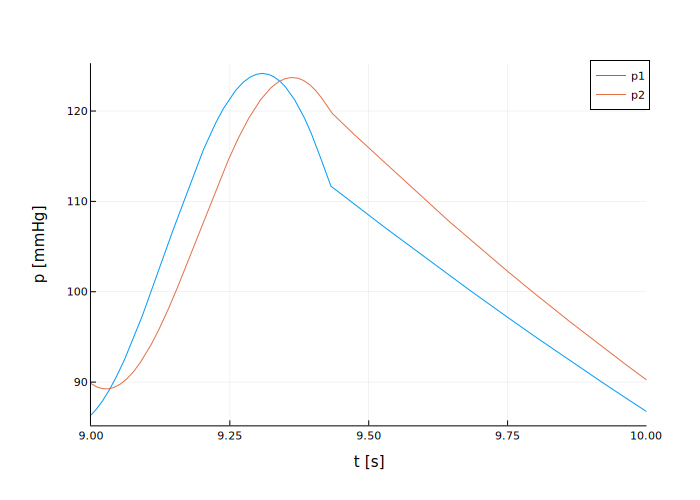
\includegraphics{ODEsolver_files/mediabag/ODEsolver_files/figure-pdf/fig-wk4-sol-output-1.pdf}

}

\end{figure}

\hypertarget{sec-odePM}{%
\subsection{Comparison to Python and Matlab}\label{sec-odePM}}

For those coming from Python or Matlab, let's have a look at how this
problem can be solved in these two languages and compare to the Julia
version.

Switch between the languages using the tabs below:

\subsection{Python}

\begin{Shaded}
\begin{Highlighting}[]
\ImportTok{import}\NormalTok{ scipy }\ImportTok{as}\NormalTok{ sp}
\ImportTok{from}\NormalTok{ scipy }\ImportTok{import}\NormalTok{ integrate}
\ImportTok{from}\NormalTok{ scipy.misc }\ImportTok{import}\NormalTok{ derivative}

\ImportTok{import}\NormalTok{ numpy }\ImportTok{as}\NormalTok{ np}

\ImportTok{import}\NormalTok{ time}

\KeywordTok{def}\NormalTok{ wk4(t, y, I, Rc, Rp, C, Lp, dt):}

\NormalTok{    dp1dt }\OperatorTok{=}\NormalTok{ (}
        \OperatorTok{{-}}\NormalTok{Rc }\OperatorTok{/}\NormalTok{ Lp }\OperatorTok{*}\NormalTok{ y[}\DecValTok{0}\NormalTok{]}
        \OperatorTok{+}\NormalTok{ (Rc }\OperatorTok{/}\NormalTok{ Lp }\OperatorTok{{-}} \DecValTok{1} \OperatorTok{/}\NormalTok{ Rp }\OperatorTok{/}\NormalTok{ C) }\OperatorTok{*}\NormalTok{ y[}\DecValTok{1}\NormalTok{]}
        \OperatorTok{+}\NormalTok{ Rc }\OperatorTok{*}\NormalTok{ derivative(I, t, dx}\OperatorTok{=}\NormalTok{dt)}
        \OperatorTok{+}\NormalTok{ I(t) }\OperatorTok{/}\NormalTok{ C}
\NormalTok{    )}

\NormalTok{    dp2dt }\OperatorTok{=} \OperatorTok{{-}}\DecValTok{1} \OperatorTok{/}\NormalTok{ Rp }\OperatorTok{/}\NormalTok{ C }\OperatorTok{*}\NormalTok{ y[}\DecValTok{1}\NormalTok{] }\OperatorTok{+}\NormalTok{ I(t) }\OperatorTok{/}\NormalTok{ C}

    \ControlFlowTok{return}\NormalTok{ [dp1dt, dp2dt]}

\NormalTok{time\_start }\OperatorTok{=} \DecValTok{0}
\NormalTok{time\_end }\OperatorTok{=} \DecValTok{10}

\NormalTok{Rc }\OperatorTok{=} \FloatTok{0.2}
\NormalTok{Rp }\OperatorTok{=} \FloatTok{1.0}
\NormalTok{C }\OperatorTok{=} \FloatTok{1.0}
\NormalTok{Lp }\OperatorTok{=} \FloatTok{1e{-}2}

\NormalTok{dt }\OperatorTok{=} \FloatTok{1e{-}6}

\NormalTok{y0 }\OperatorTok{=}\NormalTok{ np.zeros(}\DecValTok{2}\NormalTok{)}

\CommentTok{\# Generic Input Waveform}
\CommentTok{\# max volume flow in ml/s}
\NormalTok{max\_i }\OperatorTok{=} \DecValTok{425}

\CommentTok{\# min volume flow in m\^{}3/s}
\NormalTok{min\_i }\OperatorTok{=} \FloatTok{0.0}

\CommentTok{\# Period time in s}
\NormalTok{T }\OperatorTok{=} \FloatTok{0.9}

\CommentTok{\# Syst. Time in s}
\NormalTok{systTime }\OperatorTok{=} \DecValTok{2} \OperatorTok{/} \DecValTok{5} \OperatorTok{*}\NormalTok{ T}

\CommentTok{\# Dicrotic notch time}
\NormalTok{dicrTime }\OperatorTok{=} \FloatTok{0.03}

\KeywordTok{def}\NormalTok{ I(t):}
    \CommentTok{\# implicit conditional using boolean multiplicator}
    \CommentTok{\# sine waveform}
\NormalTok{    I }\OperatorTok{=}\NormalTok{ (}
\NormalTok{        (max\_i }\OperatorTok{{-}}\NormalTok{ min\_i) }\OperatorTok{*}\NormalTok{ np.sin(np.pi }\OperatorTok{/}\NormalTok{ systTime }\OperatorTok{*}\NormalTok{ (t }\OperatorTok{\%}\NormalTok{ T))}
        \OperatorTok{*}\NormalTok{(t }\OperatorTok{\%}\NormalTok{ T }\OperatorTok{\textless{}}\NormalTok{ (systTime }\OperatorTok{+}\NormalTok{ dicrTime)) }\OperatorTok{+}\NormalTok{ min\_i}
\NormalTok{    )}

    \ControlFlowTok{return}\NormalTok{ I}

\CommentTok{\# First run}
\NormalTok{tic }\OperatorTok{=}\NormalTok{ time.perf\_counter()}

\NormalTok{sol }\OperatorTok{=}\NormalTok{ sp.integrate.solve\_ivp(}
    \KeywordTok{lambda}\NormalTok{ t, y: wk4(t, y, I, Rc, Rp, C, Lp, dt),}
\NormalTok{    (time\_start, time\_end),}
\NormalTok{    y0,}
\NormalTok{    method}\OperatorTok{=}\StringTok{"RK45"}\NormalTok{,}
\NormalTok{    rtol}\OperatorTok{=}\FloatTok{1e{-}9}\NormalTok{,}
\NormalTok{    vectorized}\OperatorTok{=}\VariableTok{True}\NormalTok{,)}

\NormalTok{toc }\OperatorTok{=}\NormalTok{ time.perf\_counter()}

\BuiltInTok{print}\NormalTok{(}\SpecialStringTok{f"First run:}\CharTok{\textbackslash{}n}\SpecialStringTok{Elapsed time is }\SpecialCharTok{\{}\NormalTok{toc }\OperatorTok{{-}}\NormalTok{ tic}\SpecialCharTok{:0.4f\}}\SpecialStringTok{ seconds"}\NormalTok{)}

\CommentTok{\# Second run}
\NormalTok{tic }\OperatorTok{=}\NormalTok{ time.perf\_counter()}

\NormalTok{sol }\OperatorTok{=}\NormalTok{ sp.integrate.solve\_ivp(}
    \KeywordTok{lambda}\NormalTok{ t, y: wk4(t, y, I, Rc, Rp, C, Lp, dt),}
\NormalTok{    (time\_start, time\_end),}
\NormalTok{    y0,}
\NormalTok{    method}\OperatorTok{=}\StringTok{"RK45"}\NormalTok{,}
\NormalTok{    rtol}\OperatorTok{=}\FloatTok{1e{-}9}\NormalTok{,}
\NormalTok{    vectorized}\OperatorTok{=}\VariableTok{True}\NormalTok{,)}

\NormalTok{toc }\OperatorTok{=}\NormalTok{ time.perf\_counter()}

\BuiltInTok{print}\NormalTok{(}\SpecialStringTok{f"}\CharTok{\textbackslash{}n}\SpecialStringTok{Second run:}\CharTok{\textbackslash{}n}\SpecialStringTok{Elapsed time is }\SpecialCharTok{\{}\NormalTok{toc }\OperatorTok{{-}}\NormalTok{ tic}\SpecialCharTok{:0.4f\}}\SpecialStringTok{ seconds"}\NormalTok{)}
\end{Highlighting}
\end{Shaded}

Runtime for this code is (timed using \texttt{time.perf.counter} in
Python):

\begin{verbatim}
First run:
Elapsed time is 0.7973 seconds

Second run:
Elapsed time is 0.7810 seconds
\end{verbatim}

\subsection{MATLAB}

\begin{Shaded}
\begin{Highlighting}[]
\VariableTok{tspan} \OperatorTok{=}\NormalTok{ [}\FloatTok{0}\OperatorTok{,} \FloatTok{10}\NormalTok{]}\OperatorTok{;}

\VariableTok{Rc} \OperatorTok{=} \FloatTok{0.03}\OperatorTok{;}
\VariableTok{Rp} \OperatorTok{=} \FloatTok{1.0}\OperatorTok{;}
\VariableTok{C} \OperatorTok{=} \FloatTok{2.0}\OperatorTok{;}
\VariableTok{Lp} \OperatorTok{=} \FloatTok{1e{-}2}\OperatorTok{;}

\VariableTok{P0} \OperatorTok{=}\NormalTok{ [}\FloatTok{0}\OperatorTok{,} \FloatTok{0}\NormalTok{]}\OperatorTok{;}

\VariableTok{options}        \OperatorTok{=} \VariableTok{odeset}\NormalTok{(}\SpecialStringTok{\textquotesingle{}Reltol\textquotesingle{}}\OperatorTok{,}\FloatTok{1e{-}9}\NormalTok{)}\OperatorTok{;}

\CommentTok{\% Run once to allow Matlab to optimise}
\VariableTok{fprintf}\NormalTok{(}\StringTok{"First run:\textbackslash{}n"}\NormalTok{)}
\VariableTok{tic}
\NormalTok{[}\VariableTok{t}\OperatorTok{,} \VariableTok{P}\NormalTok{] }\OperatorTok{=} \VariableTok{ode45}\NormalTok{(}\OperatorTok{@}\NormalTok{(}\VariableTok{t}\OperatorTok{,}\VariableTok{P}\NormalTok{) }\VariableTok{wk4}\NormalTok{(}\VariableTok{t}\OperatorTok{,}\VariableTok{P}\OperatorTok{,}\VariableTok{Rc}\OperatorTok{,}\VariableTok{Rp}\OperatorTok{,}\VariableTok{C}\OperatorTok{,}\VariableTok{Lp}\NormalTok{)}\OperatorTok{,} \VariableTok{tspan}\OperatorTok{,} \VariableTok{P0}\OperatorTok{,} \VariableTok{options}\NormalTok{)}\OperatorTok{;}
\VariableTok{toc}

\CommentTok{\% Timed run}
\VariableTok{fprintf}\NormalTok{(}\StringTok{"\textbackslash{}nSecond run:\textbackslash{}n"}\NormalTok{)}
\VariableTok{tic}
\NormalTok{[}\VariableTok{t}\OperatorTok{,} \VariableTok{P}\NormalTok{] }\OperatorTok{=} \VariableTok{ode45}\NormalTok{(}\OperatorTok{@}\NormalTok{(}\VariableTok{t}\OperatorTok{,}\VariableTok{P}\NormalTok{) }\VariableTok{wk4}\NormalTok{(}\VariableTok{t}\OperatorTok{,}\VariableTok{P}\OperatorTok{,}\VariableTok{Rc}\OperatorTok{,}\VariableTok{Rp}\OperatorTok{,}\VariableTok{C}\OperatorTok{,}\VariableTok{Lp}\NormalTok{)}\OperatorTok{,} \VariableTok{tspan}\OperatorTok{,} \VariableTok{P0}\OperatorTok{,} \VariableTok{options}\NormalTok{)}\OperatorTok{;}
\VariableTok{toc}



\KeywordTok{function} \VariableTok{dP} \OperatorTok{=} \VariableTok{wk4}\NormalTok{(}\VariableTok{t}\OperatorTok{,}\VariableTok{P}\OperatorTok{,}\VariableTok{Rc}\OperatorTok{,}\VariableTok{Rp}\OperatorTok{,}\VariableTok{C}\OperatorTok{,}\VariableTok{Lp}\NormalTok{)}

\VariableTok{dP}    \OperatorTok{=} \VariableTok{zeros}\NormalTok{(}\FloatTok{2}\OperatorTok{,}\FloatTok{1}\NormalTok{)}\OperatorTok{;}

\VariableTok{dP}\NormalTok{(}\FloatTok{1}\NormalTok{) }\OperatorTok{=} \OperatorTok{{-}}\VariableTok{Rc} \OperatorTok{/} \VariableTok{Lp} \OperatorTok{*} \VariableTok{P}\NormalTok{(}\FloatTok{1}\NormalTok{) }\OperatorTok{...}
    \OperatorTok{+}\NormalTok{ (}\VariableTok{Rc} \OperatorTok{/} \VariableTok{Lp} \OperatorTok{{-}} \FloatTok{1} \OperatorTok{/} \VariableTok{Rp} \OperatorTok{/} \VariableTok{C}\NormalTok{) }\OperatorTok{*} \VariableTok{P}\NormalTok{(}\FloatTok{2}\NormalTok{) }\OperatorTok{...}
    \OperatorTok{+} \VariableTok{Rc} \OperatorTok{*} \VariableTok{didt}\NormalTok{(}\VariableTok{t}\NormalTok{) }\OperatorTok{+} \VariableTok{i}\NormalTok{(}\VariableTok{t}\NormalTok{) }\OperatorTok{/} \VariableTok{C}\OperatorTok{;}

\VariableTok{dP}\NormalTok{(}\FloatTok{2}\NormalTok{) }\OperatorTok{=} \OperatorTok{{-}}\FloatTok{1} \OperatorTok{/} \VariableTok{Rp} \OperatorTok{/} \VariableTok{C} \OperatorTok{*} \VariableTok{P}\NormalTok{(}\FloatTok{2}\NormalTok{) }\OperatorTok{+} \VariableTok{i}\NormalTok{(}\VariableTok{t}\NormalTok{) }\OperatorTok{/} \VariableTok{C}\OperatorTok{;}

\KeywordTok{end}

\KeywordTok{function} \VariableTok{i} \OperatorTok{=} \VariableTok{i}\NormalTok{(}\VariableTok{t}\NormalTok{)}

\VariableTok{max\_i} \OperatorTok{=} \FloatTok{425}\OperatorTok{;}
\VariableTok{min\_i} \OperatorTok{=} \FloatTok{0.0}\OperatorTok{;}

\VariableTok{T} \OperatorTok{=} \FloatTok{0.9}\OperatorTok{;}

\VariableTok{systTime} \OperatorTok{=} \FloatTok{2} \OperatorTok{/} \FloatTok{5} \OperatorTok{*} \VariableTok{T}\OperatorTok{;}

\VariableTok{dicrTime} \OperatorTok{=} \FloatTok{0.03}\OperatorTok{;}

\VariableTok{i} \OperatorTok{=}\NormalTok{ ((}\VariableTok{max\_i} \OperatorTok{{-}} \VariableTok{min\_i}\NormalTok{) }\OperatorTok{*} \VariableTok{sin}\NormalTok{(}\VariableTok{pi} \OperatorTok{/} \VariableTok{systTime} \OperatorTok{*}\NormalTok{ (}\VariableTok{mod}\NormalTok{(}\VariableTok{t}\OperatorTok{,}\VariableTok{T}\NormalTok{))) }\OperatorTok{...}
    \OperatorTok{*}\NormalTok{(}\VariableTok{mod}\NormalTok{(}\VariableTok{t}\OperatorTok{,}\VariableTok{T}\NormalTok{) }\OperatorTok{\textless{}}\NormalTok{ (}\VariableTok{systTime} \OperatorTok{+} \VariableTok{dicrTime}\NormalTok{)) }\OperatorTok{...}
    \OperatorTok{+} \VariableTok{min\_i}\NormalTok{)}\OperatorTok{;}

\KeywordTok{end}

\KeywordTok{function} \VariableTok{didt} \OperatorTok{=} \VariableTok{didt}\NormalTok{(}\VariableTok{t}\NormalTok{)}
\VariableTok{dt} \OperatorTok{=} \FloatTok{1e{-}3}\OperatorTok{;}
\VariableTok{didt} \OperatorTok{=}\NormalTok{ (}\VariableTok{i}\NormalTok{(}\VariableTok{t}\OperatorTok{+}\VariableTok{dt}\NormalTok{) }\OperatorTok{{-}} \VariableTok{i}\NormalTok{(}\VariableTok{t}\OperatorTok{{-}}\VariableTok{dt}\NormalTok{)) }\OperatorTok{/}\NormalTok{ (}\FloatTok{2} \OperatorTok{*} \VariableTok{dt}\NormalTok{)}\OperatorTok{;}
\KeywordTok{end}
\end{Highlighting}
\end{Shaded}

Runtime for this code is (timed using \texttt{tic} \texttt{toc} in
Matlab)\sidenote{\footnotesize Same code in Octave, the free open-source version of
  Matlab runs in 3 seconds. Current versions of Matlab have improved
  runtime by partial just-in-time compilation. Note that the first run
  in Matlab also takes an order of magnitude longer, which is most
  likely due to Matlab optimising the solver to the problem.}, which is
a bit more than an order of magnitude slower than Julia:

\begin{verbatim}
First run:
\end{verbatim}

\begin{verbatim}
Elapsed time is 0.363712 seconds.

Second run:
Elapsed time is 0.032150 seconds.
\end{verbatim}

So in this case, Julia is one order of magitude faster than Matlab and
around 500x faster than Python\sidenote{\footnotesize I have tried using PyPy and
  Cython in other cases and found that they speed up Python
  considerably. Unfortunately this was not the case when using SciPy and
  Numpy, which made the compiled Python version one order of magnitude
  \textbf{slower} than interpreted. There seems to be a problem with
  C-calls from PyPy.} solving ODEs.

Personally, I find the Matlab code and, in particular, the Julia code
easier to read.




\end{document}
